This chapter discusses how we set up the user evaluation, what we evaluated, and how the results were. Additionally, the analysis of the evaluation's results is provided.


\section{User Evaluation}

User evaluation is a method of testing and assessing a system that involves giving users access to the system and asking for their feedback after using. For this prototype, we aimed to evaluate its functionality and usability using tasks and questionnaires. We then collected the feedback and results to calculate user performance, functionality, and usability scores; and interpreted what the scores could imply. 

All participants were recruited by being invited or self-volunteering through the recruiting email. Each participant had to read and agree to the participant's information sheet and consent form.
% , which are provided in the Appendix chapters \ref{pis} and \ref{pcf}
Moreover, no personal information was collected, so there was no privacy violation in this study.

We collected three pieces of information from participants: task results, questionnaire responses, and feedback.
To collect responses and feedback, we created a Google form that contained scenarios, tasks, and questionnaires.
% which can be seen in Appendix \ref{appendeix_evaluation}.
Each scenario had tasks to generate a specific checklist. To perform each task and collect its result, participants needed to go to the prototype's website to complete those tasks. After submitting the tasks, participants would be asked to fill out questionnaires and an optional open-ended feedback question at the end.

\subsection{Setup}
Before we recruited people to evaluate the prototype, we needed to set up the system so that participants could visit the prototype and complete the tasks. We implemented a separate route on the frontend\footnote{\href{https://resource-based-checklist-generation.vercel.app/evaluation}{https://resource-based-checklist-generation.vercel.app/evaluation}} for this evaluation.
Upon arriving at the evaluation route, an evaluation code was generated to link the results of each task with the questionnaires for further analysis, which we will discuss in Section \ref{eval:results}.
% The results were collected once participants completed each task.
% Each screen was a canvas screen with the scenario and the objective of the task that participants needed to perform.
% This facilitated participants by not having to switch back and forth between the prototype's website and the Google Form.

\subsection{Scenarios and Tasks}
% As mentioned in the introduction of this section, we designed two scenarios for this user evaluation.
We designed two scenarios for participants to perform.
The first scenario was a payment process with an order detail as the input and debit card information as the output. The second scenario was a healthcare process with a treatment contract and doctor information as the input and an updated contract as the output. Both scenarios are provided in Appendix \ref{appendeix_evaluation}.
% Please refer to Appendix \ref{appendeix_evaluation} for more details.
% The first scenario included instructions to help participants get used to the system, while the second scenario did not.

% The first scenario was, \textit{``You are a checklist designer for a payment workflow. The owner wants you to create a checklist template for a CardInput process. In this process, a customer needs to enter the credit/debit card number, expire date, and security code to pay for some purchased items. The process contains OrderTransaction as the input information, with fields as described below. Additionally, the output form needs to be linked with the CardDetails output of the workflow process."}

The purpose of the first scenario was to help participants get used to the system.
Participants were to perform two tasks in this scenario. The first task was to create a checklist based on the first scenario without using any assisting features (\textbf{Auto-Generation} and \textbf{Query Suggestion}). The second task was to create the exact same checklist; however, participants were allowed to use the assisting features. This was to evaluate how good the assisting features were in improving the accuracy of creating a checklist based on the user performance scores. In addition, each task included instructions to guide participants on what to do to complete each task.

% The second scenario was, \textit{``You are a checklist designer for a healthcare workflow. A doctor asks you to create a checklist template for an AwardContract process. In this process, a clinician agrees to another member of clinical staff, (the ServiceProvider) to provide a medical service on their behalf (i.e. delegating the task to someone else). The process contains two useful pieces of input information: the ServiceProvider that contains information on the doctor who is assigned to the contract, and AcceptedContract that contains information about the contract itself (i.e. the nature of the clinical task, details about the patient, etc)."}

In the second scenario, participants were to perform only one task. Much like the first two tasks, the third task was to generate a checklist based on the second scenario. However, no instructions were provided for this task. This was because we wanted to measure how well participants would perform after becoming familiar with the system.

% The second scenario contained only one task without any instructions provided. The task in this scenario was more difficult than the previous tasks to evaluate how 

\subsection{Questionnaires}
We decided to make two questionnaires to gather participant feedback: functionality and usability.
Each question in the questionnaires contained five response options, from disagree (1) to agree (5).
The functionality questionnaire was designed to evaluate the core features when creating a checklist | including \textbf{Input Information Query}, \textbf{Form Adjustment}, \textbf{Dependency Linkage}; and the usefulness of the assisting features.
The list of questions can be seen in Appendix \ref{appendix:questionnaire}.

% The second functionality questionnaire was asked at the end of the evaluation. This questionnaire aimed to collect feedback on how helpful the assisting features were in helping complete the task without any instructions.
% The list of questions can be seen in Appendix \ref{appendix:questionnaire}.


The usability questionnaire followed the standard usability questionnaire by John Brooke \cite{susscores} with two additional questions. That is because Brooke's usability questionnaire allowed us to convert the responses to the System Usability Scale (SUS) score, which can be interpreted later on. The two extra questions were added to evaluate the complexity of the system after learning through instructions and the convenience of using the assisting features in creating a checklist.
The list of questions can be seen in Appendix \ref{appendix:questionnaire}.


\section{Results}
\label{eval:results}
We ultimately recruited 13 participants to take part in this evaluation.
Functionality scores, SUS score, and performance accuracy will be discussed in this section.
% Questionnaire scores and accuracy are the two metrics that we will discuss in this section.

% At the end, we recruited 13 participants to evaluate this project.
% As mentioned earlier, we collected task results, questionnaire responses, and feedback from the participants. In this section, we calculated and summarised the data into two metrics: accuracy and scores.

\subsection{Functionality Scores}
\label{eval:func_scores}
Functionality scores are calculated using responses to the functionality questionnaire, arranging from the lowest score of 1 to the highest score of 5. This can be grouped into four categories according to the features being evaluated in this questionnaire (\textbf{Input Information Query}, \textbf{Form Adjustment}, \textbf{Dependency Linkage}, and the usefulness of the assisting features), as shown in Table \ref{tab:func_scores} | the full score distribution for each question is provided in Appendix \ref{appendix:questionnaire_scores}.


\begin{table}[ht!]
    \centering
    \footnotesize
    \begin{tabular}{
      |p{\dimexpr.35\linewidth-2\tabcolsep-1.3333\arrayrulewidth}% column 1
      |p{\dimexpr.15\linewidth-2\tabcolsep-1.3333\arrayrulewidth}% column 2
      |p{\dimexpr.15\linewidth-2\tabcolsep-1.3333\arrayrulewidth}|% column 3
      }
      \hline
      \centering Features & \centering Mean & \centering\arraybackslash SD    \\ \hline
      \hfil \textbf{Input Information Query} & \hfil 3.88 & \hfil 0.99 \\ \hline
      \hfil \textbf{Form Adjustment} & \hfil 4.04 & \hfil 0.8 \\ \hline
      \hfil \textbf{Dependency Linkage} & \hfil 4.23 & \hfil 0.93 \\ \hline
      \hfil Assisting features & \hfil 4.23 & \hfil 0.99 \\ \hline
    \end{tabular}
    \caption{Functionality Scores}
    \label{tab:func_scores}
\end{table}

From the scores in Table \ref{tab:func_scores}, we can see that, on average, the functionality scores are fairly high. This implies that the participants were able to use these functionalities successfully.
It is noteworthy that the functionality score for \textbf{Input Information Query} is significantly lower when compared to other features. According to participant feedback, the \textbf{Input Information Query} feature was not clear because this feature was hidden behind the ellipsis in the input information section.
% This is a constructive criticism that can be improved upon in future work.

Another interesting point to make is, participants gave an average score of 4.46 for the convenience question\footnote{The convenience of using the assisting features in creating a checklist} | one of the extra questions in the usability questionnaire. This implies that the assisting features (\textbf{Auto-Generation} and \textbf{Query Suggestion}) make the process of creating a checklist much easier. This point will be further discussed in more detail in Section \ref{eval:acc}.


\subsection{SUS Score}
\label{eval:sus_score}
The System Usability Scale (SUS) score is a measurement method created by John Brooke \cite{susscores} to calculate a standard score which implies how good a system is via ten usability questions. According to Lewis' work \cite{68avgsus}, the average SUS score of over 500 studies is 68.

Our system got a SUS score of 63.08. This score is considered below average, as mentioned earlier. However, as we inspected the score distribution | which can be seen in Appendix \ref{appendix:questionnaire_scores}, we found that our system received relatively low scores on the complexity part of the questionnaire. To emphasise this point, a good amount of participant feedback mentioned that the explanation of the whole system in the user evaluation was not enough for them to be able to understand what the system was.

This was to be expected because this system is conceptually complex and requires a lot of background knowledge to understand what is going on, such as BPM, WorkflowFM, checklists, etc. Especially, we had to consider the amount of information in the evaluation was not too lengthy so that participants would not feel overwhelmed.
% This created a gap understanding of what was going on during the task performance.
% improvement


% The SUS score can be interpreted by measuring the score against Bangor's adjective rating scale \cite{bangor2009determining}, as shown in Figure \ref{fig:adjective-ratings}.

% \begin{figure}[ht!]
%     \centering
%     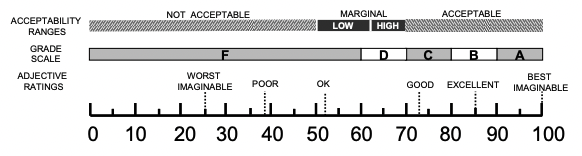
\includegraphics[width=0.9\textwidth]{overleaf/images/adjective-ratings (1).png}
%     \caption{Bangor's Adjective Ratings \cite{bangor2009determining}}
%     \label{fig:adjective-ratings}
% \end{figure}



\subsection{Performance Accuracy}
\label{eval:acc}
We collected the results of each task from the participants and called them user performance results. User performance results were used to calculate the accuracy scores by checking the results against the expected answer.

\begin{table}[ht!]
    \centering
    \footnotesize
    \begin{tabular}{
      |p{\dimexpr.25\linewidth-2\tabcolsep-1.3333\arrayrulewidth}% column 1
      |p{\dimexpr.15\linewidth-2\tabcolsep-1.3333\arrayrulewidth}% column 1
      |p{\dimexpr.15\linewidth-2\tabcolsep-1.3333\arrayrulewidth}|% column 3
      }
      \hline
      \centering Tasks & \centering Accuracy & \centering\arraybackslash  Time Taken   \\ \hline
      \hfil \#1 (First Scenario) & \hfil 0.86 & \hfil 15:24 \\ \hline
      \hfil \#2 (First Scenario) & \hfil 0.90 & \hfil 05:51 \\ \hline
      \hfil \#3 (Second Scenario) & \hfil 0.91 & \hfil 12:54 \\ \hline
    \end{tabular}
    \caption{Performance Accuracy and Time Taken}
    \label{tab:user_performance}
\end{table}

As seen in Table \ref{tab:user_performance}, the accuracy scores are remarkably high. This implies that the participants were able to successfully perform the tasks despite them not understanding the context of the system, as mentioned in Section \ref{eval:sus_score}. This also corresponds to one of the points in Section \ref{eval:func_scores} that the assisting features make the process of creating a checklist so much easier that participants do not need to understand the context of the system to perform the tasks correctly.

It is also interesting to look at the time taken on average in Table \ref{tab:user_performance}. That is because the time difference between task 1 and task 2 is significantly huge. This could be interpreted two ways: 1.) since the second task was similar to the first task, participants did not need to go through the scenario again to perform this task; 2.) the assisting features significantly reduced the amount of time taken to create checklists.

Regarding our opinions, we speculated that both hypotheses could be true. That was because while the first and second tasks shared the same scenario, the amount of time deducted was so significant that this could not be the only reason that caused this circumstance. Additionally, due to the fact that functionality scores on the assisting feature-related questions were remarkably high, this supports the second hypothesis. With the current data, we could not objectively say that the second hypothesis is definitely true, but it is most likely to be.

% \section{Comparison with Existing Tools}

% \section{Test Scenarios}
% \subsection{Healthcare Scenarios}
% \begin{figure}[ht]
%     \centering
%     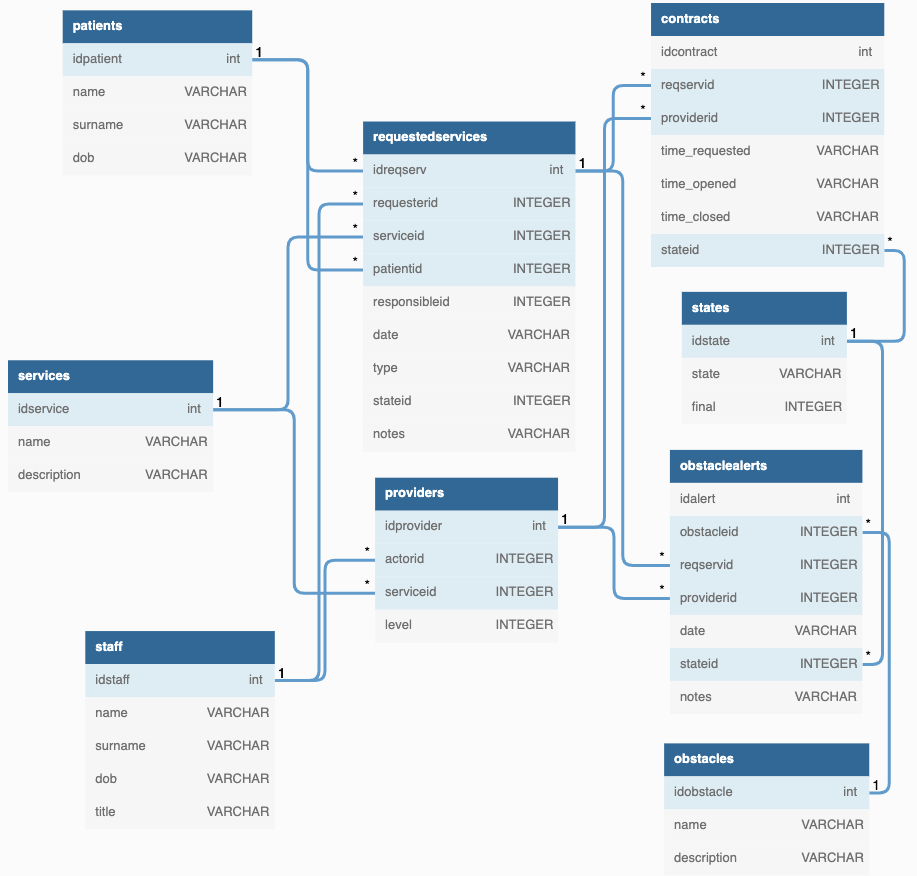
\includegraphics[width=\textwidth]{overleaf/images/chens_healthcare_db_design.png}
%     \caption{Chen's Healthcare Database Design}
%     \label{fig:chens_healthcare_db_design}
% \end{figure}

% \subsection{Payment Scenarios}

% handle array since healthcare does not have array type input

% \begin{figure}[ht]
%     \centering
%     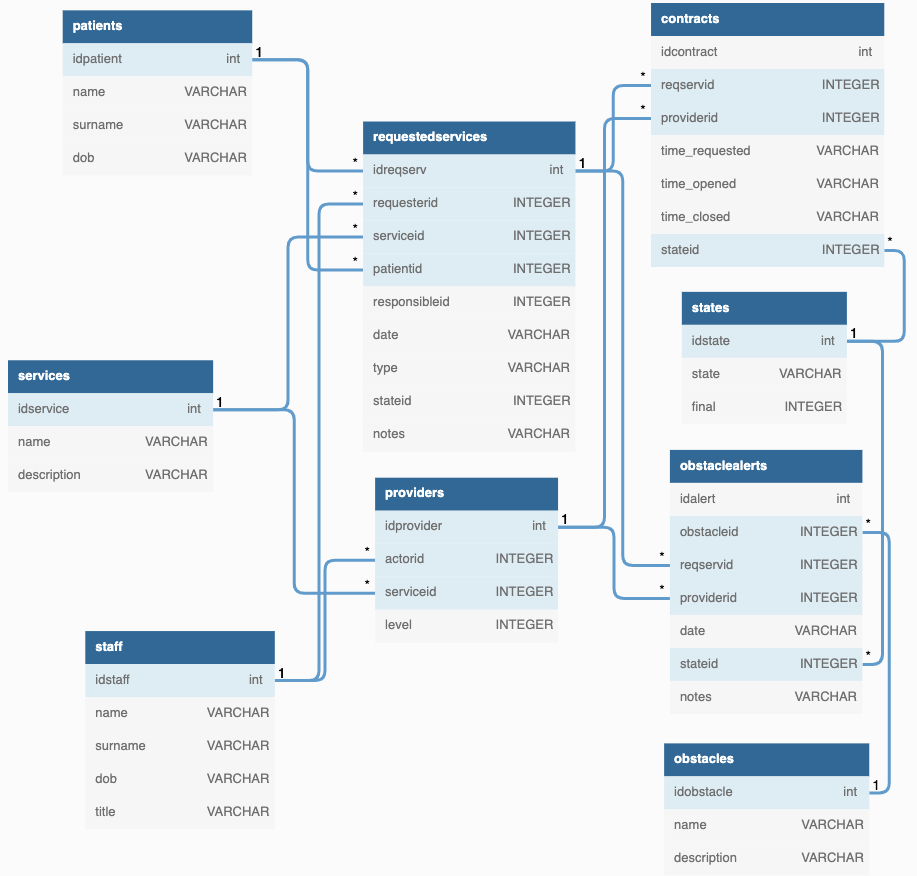
\includegraphics[width=\textwidth]{overleaf/images/chens_healthcare_db_design.png}
%     \caption{Payment Database Design}
%     \label{fig:payment_db_design}
% \end{figure}

% \section{Questionnaire}
% \subsection{Tasks}
% \subsection{Questions}
% \subsection{Results}

% \section{Unit Testing}
% \subsection{Results}

% \section{Improvement}
% precision-recall, and analysis from the result to develop helping tools